%!TEX program = xelatex

\documentclass[a4paper, openany, oneside]{memoir}
\usepackage[no-math]{fontspec}
\usepackage{pgfplots}
\pgfplotsset{compat=newest}
\usepackage{commath}
\usepackage{mathtools}
\usepackage{amssymb}
\usepackage{amsthm}
\usepackage{booktabs}
\usepackage{mathtools}
\usepackage{xcolor}
\usepackage[separate-uncertainty=true, per-mode=symbol]{siunitx}
\usepackage[noabbrev, capitalize]{cleveref}
\usepackage{listings}
\usepackage[american inductor, european resistor]{circuitikz}
\usepackage{amsmath}
\usepackage{amsfonts}
\usepackage{ifxetex}
\usepackage[dutch,english]{babel}
\usepackage[backend=bibtexu,texencoding=utf8,bibencoding=utf8,style=ieee,sortlocale=en_GB,language=auto]{biblatex}
\usepackage[strict,autostyle]{csquotes}
\usepackage{parskip}
\usepackage{import}
\usepackage{standalone}
\usepackage{hyperref}
%\usepackage[toc,title,titletoc]{appendix}

\ifxetex{} % Fonts laden in het geval dat je met Xetex compiled
    \usepackage{fontspec}
    \defaultfontfeatures{Ligatures=TeX} % To support LaTeX quoting style
    \setromanfont{Palatino Linotype} % Tover ergens in Font mapje in root.
    \setmonofont{Source Code Pro}
\else % Terug val in standaard pdflatex tool chain. Geen ondersteuning voor OTT fonts
    \usepackage[T1]{fontenc}
    \usepackage[utf8]{inputenc}
\fi
\newcommand{\references}[1]{\begin{flushright}{#1}\end{flushright}}
\renewcommand{\vec}[1]{\boldsymbol{\mathbf{#1}}}
\newcommand{\uvec}[1]{\boldsymbol{\hat{\vec{#1}}}}
\newcommand{\mat}[1]{\boldsymbol{\mathbf{#1}}}
\newcommand{\fasor}[1]{\boldsymbol{\tilde{\vec{#1}}}}
\newcommand{\cmplx}[0]{\mathrm{j}}
\renewcommand{\Re}[0]{\operatorname{Re}}
\newcommand{\Cov}{\operatorname{Cov}}
\newcommand{\Var}{\operatorname{Var}}
\newcommand{\proj}{\operatorname{proj}}
\newcommand{\Perp}{\operatorname{perp}}
\newcommand{\col}{\operatorname{col}}
\newcommand{\rect}{\operatorname{rect}}
\newcommand{\sinc}{\operatorname{sinc}}
\newcommand{\IT}{\operatorname{IT}}
\newcommand{\F}{\mathcal{F}}

\newtheorem{definition}{Definition}
\newtheorem{theorem}{Theorem}


\DeclareSIUnit{\voltampere}{VA} %apparent power
\DeclareSIUnit{\pii}{\ensuremath{\pi}}

\hypersetup{%setup hyperlinks
    colorlinks,
    citecolor=black,
    filecolor=black,
    linkcolor=black,
    urlcolor=black
}

% Example boxes
\usepackage{fancybox}
\usepackage{framed}
\usepackage{adjustbox}
\newenvironment{simpages}%
{\AtBeginEnvironment{itemize}{\parskip=0pt\parsep=0pt\partopsep=0pt}
\def\FrameCommand{\fboxsep=.5\FrameSep\shadowbox}\MakeFramed{\FrameRestore}}%
{\endMakeFramed}

% Impulse train
\DeclareFontFamily{U}{wncy}{}
\DeclareFontShape{U}{wncy}{m}{n}{<->wncyr10}{}
\DeclareSymbolFont{mcy}{U}{wncy}{m}{n}
\DeclareMathSymbol{\Sha}{\mathord}{mcy}{"58}
\addbibresource{../../includes/bibliography.bib}

\begin{document}

\section{Introduction}

\cref{cha:sampling,cha:reconstruction,cha:sampling_methods,cha:detection} have analysed and described several
sampling, reconstruction and detection techniques. It is in this chapter that we will evaluate their performance such that a discussion and a conclusion can be draw based on the specifications as described \cref{sec:theory-specs}. This chapter will start with an overview of the complete system, to continue with a description of the tests performed to assess the performance of this system. This chapter will end with the results
of those tests which will be discussed in \textbf{verwijs naar discussie chapter}.

\section{Overview}
A block diagram of the complete system is depicted in \cref{fig:theoretical_overview_system}. Considered options that did not make it into
the final system are grayed out. 

\begin{figure}[H]
\centering
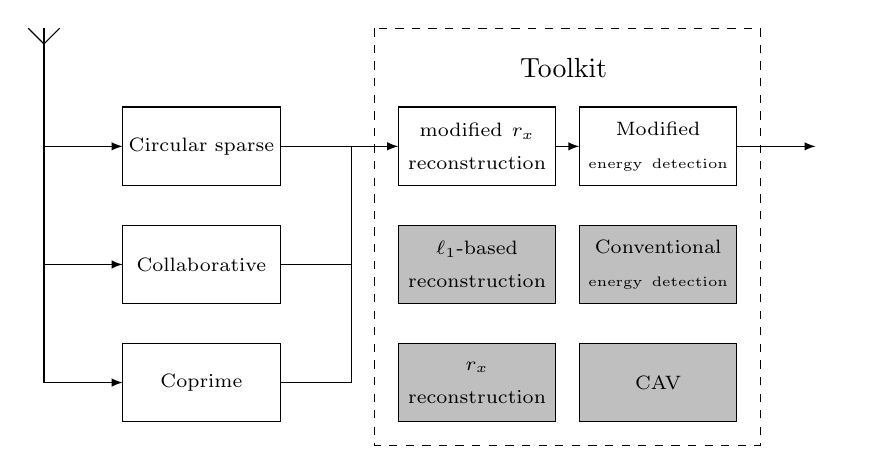
\begin{tikzpicture}
\draw  (-2,3) rectangle (0,2) node[pos=.5]{\scriptsize Circular sparse};
\draw  (-2,1.5) rectangle (0,0.5) node[pos=.5]{\scriptsize Collaborative};
\draw  (-2,0) rectangle (0,-1) node[pos=.5]{\scriptsize Coprime};
\draw  (1.5,3) rectangle (3.5,2) node[text width=5cm, align=center,pos=.5]{\scriptsize modified $r_x$\\ reconstruction};
\draw  [fill=lightgray] (1.5,0) rectangle (3.5,-1) node[text width=5cm, align=center,pos=.5]{\scriptsize $r_x$\\ reconstruction};
\draw  [fill=lightgray](1.5,1.5) rectangle (3.5,0.5) node[text width=5cm, align=center,pos=.5]{\scriptsize $\ell_1$-based\\ reconstruction};
\draw  (3.8,3) rectangle (5.8,2) node[text width=5cm, align=center,pos=.5]{\scriptsize Modified\\\tiny energy detection};
\draw  [fill=lightgray] (3.8,1.5) rectangle (5.8,0.5) node[text width=5cm, align=center,pos=.5]{\scriptsize Conventional\\\tiny energy detection};
\draw  [fill=lightgray](3.8,0) rectangle (5.8,-1) node[pos=.5]{\scriptsize CAV};
\draw  [dashed] (1.2,4) rectangle (6.1,-1.3);
\node at (3.6,3.5) {Toolkit};
\draw [>=latex,->] (3.5,2.5) -- (3.8,2.5);
\draw [>=latex,->] (5.8,2.5) -- (6.8,2.5);
\draw [>=latex,->] (0,2.5) -- (1.5,2.5);
\draw [>=latex,->] (-3,2.5) -- (-2,2.5);
\draw [>=latex,->] (-3,1) -- (-2,1);
\draw [>=latex,->] (-3,-0.5) -- (-2,-0.5);
\draw (0,-0.5) -- (0.9,-0.5);
\draw (0,1) -- (0.9,1);
\draw (-3,-0.5) -- (-3,4);
\draw (0.9,-0.5) -- (0.9,2.5);
\draw (-2.8,4) -- (-3,3.8);
\draw (-3.2,4) -- (-3,3.8);
\node at (3.5,3) {};
\end{tikzpicture}
\caption{Overview of complete system \& design choices}
\label{fig:theoretical_overview_system}
\end{figure}

\section{Testing}
To evaluate the performance of our system we will we use an artificial testing signal to test both the reconstructor and the detector.
Details on this signal generation can be found in \cref{ssec:test_signal}.

\subsection{Test signal}\label{ssec:test_signal}
To construct the testing signal given a desired SNR we take the following steps:

\begin{enumerate}
	\item Generate the signal $s[n]$ which is done by generating circular symmetric complex gaussian noise and filtering it such that it represents a bandpass signal with $-0.4\pi \leq \Omega \leq 0.4\pi$. The average power of the signal at frequencies in the passband is chosen such
	that the required SNR will be met. 
	\item Generate the additive circular symmetric complex gaussian noise signal $w[n]$ 
	\item Add $s[n]$ to $w[n]$ to produce the testing signal $x[n]$
\end{enumerate}



\subsection{Tests}
There are four parameters of the system, circled in \cref{tkz:test_system}, that will be used in our tests to asses the performance of the system:
\begin{enumerate}
	\item SNR of the input signal.
	\item The sampler type used to sample the input signal.
	\item The false alarm probability $p\ss{fa}$ of the detector.
\end{enumerate}

\begin{figure}[H]
\centering
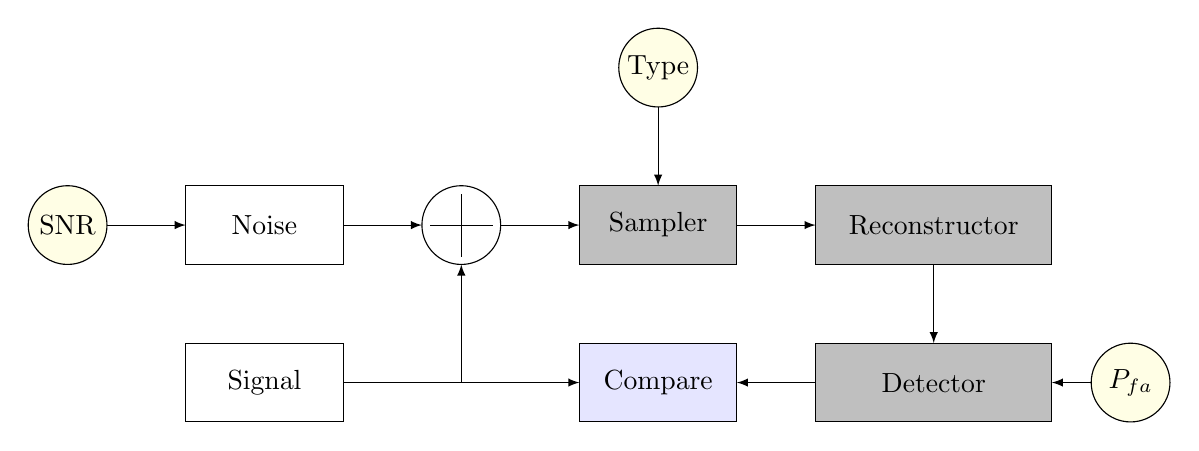
\begin{tikzpicture}

\draw  (-2,3.5) rectangle (0,2.5) node[pos=.5]{Noise};
\draw  (-2,1.5) rectangle (0,0.5) node[pos=.5]{Signal};
\draw  (1.5,3) ellipse (.5 and .5);
\draw  [fill=lightgray](3,3.5) rectangle (5,2.5) node[pos=.5]{Sampler};
\draw  [fill=lightgray](6,3.5) rectangle (9,2.5) node[pos=.5]{Reconstructor};
\draw  [fill=lightgray](6,1.5) rectangle (9,0.5) node[pos=.5]{Detector};
\draw  [fill=blue, opacity=.1](3,1.5) rectangle (5,0.5);
\draw  (3,1.5) rectangle (5,0.5)node[pos=.5]{Compare};



\draw (1.5,2.6) -- (1.5,3.4);
\draw (1.9,3) -- (1.1,3);
\draw [>=latex, ->] (0,3) -- (1,3);
\draw [>=latex, ->] (9.5,1) -- (9,1);
\draw [>=latex, ->] (4,4.5) -- (4,3.5);
\draw [>=latex, ->] (1.5,1) -- (1.5,2.5);
\draw [>=latex, ->] (-3,3) -- (-2,3);
\draw [>=latex, ->] (6,1) -- (5,1);
\draw [>=latex, ->] (0,1) -- (3,1);
\draw [>=latex, ->] (7.5,2.5) -- (7.5,1.5);
\draw [>=latex, ->] (2,3) -- (3,3);
\draw [>=latex, ->] (5,3) -- (6,3);


\draw   [fill=yellow, opacity=.1] (-3.5,3) ellipse (.5 and .5);
\draw   [fill=yellow, opacity=.1] (10,1) ellipse (.5 and .5);

\draw   [fill=yellow, opacity=.1] (4,5) ellipse (.5 and .5);

\draw   (-3.5,3) ellipse (.5 and .5) node{SNR};
\draw  (10,1) ellipse (.5 and .5) node{$P_{fa}$};

\draw  (4,5) ellipse (.5 and .5) node{Type};

\end{tikzpicture}
\caption{Testing the system}\label{tkz:test_system}
\end{figure}

Our tests will be targeted at
\begin{enumerate}
	\item adressing the performance of the reconstruction and feeding it an artificial constructed signal while
	\begin{enumerate}
		\item varying the sampling technique used to sample the signal (as described in \cref{cha:sampling_methods});
		\item varying the compression rate and the oversampling factor (as described in \cref{cha:reconstruction}).
	\end{enumerate}
	By comparing the reconstructed the power spectral density to the power spectral density recovered directly from the constructed test signal, we can evaluate the correctness of reconstruction when used with a specific sampling technique.
	Furthermore the dependence on the oversampling factor and the compression factor can be evaluated from those test results. 
	\item adressing the performance of detection on the reconstructed signal. The energy detector as described in \cref{ssec:ari_ed} will be evaluated by tests that make use of the test signal as described in \cref{ssec:test_signal}. 
	The detector is applied to the output of the reconstructor while	
	\begin{enumerate}
		\item varying the signal-to-noise ratio of the test signal; 
		\item varying the false alarm probability the detector 
		should allow;
		\item varying the compression rate of the reconstructor.
	\end{enumerate}
	Using these results we can construct the receiver operating characteristic curves (ROC-curves) which plot the detection probability versus the false alarm probability of the detector. From these curves the minimum signal strength and the detectors performance on a random signal can be evaluated. Furthermore the detection performance of the system as a whole can be evaluated by comparing these curves for different compression rates.
	\end{enumerate}

\section{Results}

\begin{filecontents*}{plots/plot-data.csv}
x, y
1, 1
2, 3
3, 4
4, 3
\end{filecontents*}
\begin{figure}
	\centering
	\begin{tikzpicture}
		\begin{axis}[
				xlabel={Sampling time at 25 MHz (ms)},
				ylabel={Normalised mean squared error of PSD ($\log_{10}$)},
				width=8cm,
				height=8cm,
				scale=1,
				grid=both,
				axis lines=left
			]
		    \addplot [
			    color=red,
			    solid,
			    mark=o
		    ] table [x=x, y=y, col sep=comma]{plots/plot-data.csv};
		\end{axis}
	\end{tikzpicture}
	\caption{test}
	\label{fig:plot}
\end{figure}



\section{Discussion: keesch}
For circular sparse ruler we constructed solutions with higher performance than proposed in \cite{ariananda2012compressive}. Our method is a novelty and contributes to higher efficiency in our product. We also made an recursive algorithm to generate circular sparse ruler solutions,  but this was a less clean approach, because it used  theorys we could not prove, and therefore did not guarantee to find the best solutions. Overall we managed to get a lot of efficiency out of the sampling techniques, but we cannot know for sure whether a more efficient solution is possible or not.

We implemented three sampling methods that are quite different and fit them into our system. This shows potential for a more general sampling technique. For instance: what happens when we combine multiple coprime devices, or what happens when we pick the circular sparse ruler problem, and allow the sampling frequency to differ. There is potential to look fo a more general sampling strategy but investigating this further needs future work.

This also holds for optimisation strategies. It would be very interesting to compare the different optimisation strategies and see whether they can benefit from each other. The collaborative sampler has for example currently no good algorithm to find configurations for more than two devices with more than three samplers. 

In this section we saw the sampling strategies grow towards each other and it would be interesting to see what happens if they move even further towards each other in the future. 

For collaborative sampling we looked at a method where the different devices are used to sense more bandwidth, but collaborative sampling can also be used for other purposes, like increasing accuracy, or sensing in a larger radius. We did not look at these applications and this should be considered future work.



\end{document}
